\documentclass[12pt,a4paper, twocolumn, twoside]{article}
\usepackage{amsmath}
\usepackage[english]{babel}
\usepackage{graphicx}
\usepackage{caption}
\usepackage{subcaption}
\usepackage{xcolor}
\usepackage{float}

\newcommand{\diff}[2]{\frac{\partial{#1}}{\partial{#2}}}
\newcommand{\todo}{\textcolor{red}{\textbf{TODO:}}}

\begin{document}
	
	\title{Task priority assignment with collision avoidance.}
	\author{Stefano De Filippis \& Marco Menchetti}
	\date{October 2019}
	\maketitle
	
\begin{abstract}
	\textbf{
	In this paper we will face the problem of task priority resolution using a fast computation of the priority matrix (here \textit{Flacco Matrix}) and the resulting joint velocities.}

\textbf{
	Collision avoidance for several control points has been taken as a high priority task in this case as well as trajectory tracking.}
\end{abstract}
%\begin{keywords}
%	Priority; Task Priority; Collision Avoidance	
%\end{keywords}
\section*{Introduction}
Due to their high dexterity and the absence of non-holonomic constraints, manipulators has been used to perform a wide range of operation, and sometimes even more of them at the same time.

A handy yet practical example is the one considered below: a manipulator moving in a cluttered environment, trying to complete a trajectory tracking task and, at the same time, avoid collision with obstacles nearby.

\section{Tasks definition}
The tasks we used are four and they occupy all 7 manipulator's DOF:
\begin{itemize}
	\item one cartesian positioning task occupying 3 DOF.
	\item one cartesian orientation task for the second link, which occupies 2 DOF.
	\item two control points' collision avoidance tasks that will occupy overall 2 DOF.
\end{itemize}
\subsection[Task 1]{cartesian positioning}
The cartesian positioning task is defined by the direct kinematics of the robot, $f(q)$, so the \textbf{end-effector}'s position is $r = f(q)$. Hence it's straight-forward the expression of this task's velocity with respect to the joints' one: 
\begin{equation}
\label{EQN: task1}
 \dot{r} = \diff{f(q)}{q} \dot{q} = J\dot{q}
\end{equation}

\subsubsection{Collision avoidance}
In the formulation of our problem, where $\dot{r}$ is given (i.e. precalculated), we are left with finding the right value for $\dot{q}$.

As already said, in our approach, we have also to include the collision avoidance for the end-effector. Instead of treating it as a different task, as we will do for the other control points, we could handle it in a "tricky" way so as to not saturate other DOFs: we will use instead of $\dot{r}$, the \textbf{sum} between $\dot{r}$ and another cartesian velocity pushing the end-effector away from the obstacle. This cartesian velocity will be (or \todo add citation i.e. as in [1])directed as the distance from the center of the obstacle to the tip of the manipulator, and will have a magnitude weighted by a non-linear gain $v(P,O)$, where $P = f(q)$ is the end-effector position and $O$ is the obstacle position.
Hence:
\begin{equation}\label{repulsive_dir}
\dot{r_o} = v(P,O)\frac{f(q) - O}{\lVert f(q) - O \rVert}
\end{equation}
\begin{equation}\label{repulsive_mag}
v(P,O) = \frac{V_{max}}{1+e^{(\lVert f(q) -O \rVert(2/\rho)-1)\alpha}}
\end{equation}

In the end we will have \eqref{EQN: task1} in the form: 
\[
\dot{r} + \dot{r_o} = J\dot{q}
\]
\subsection[Task 2]{Cartesian orientation}
\todo all again and check if the equation is right
\subsection[Tasks 3 \& 4]{Control points' collision avoidance}
When dealing with the collision avoidance task linked to the two control points we were left with only 2 DOFs for both so we had to use one for each point. We couldn't use the same approach we used for the end-effector but at the same time something rather similar has to be done. 

To compress the three DOFs into one, we projected the collision avoidance task velocity, $\mathbf{\dot{r_{o}}_{,i}}$ computed as in \eqref{repulsive_dir} but using the control point position as $P$, onto the direction of the velocity itself. In this way we get a task velocity which is a scalar (1 DOF) equal to the magnitude of the original one (i.e. \eqref{repulsive_mag}).

Defining 
\begin{itemize}
	\item $\eta = \frac{P - O}{\lVert P-O \rVert}$
	\item $P$ as the control point's position
	\item $O$ as the position of the obstacle
	\item $J_i$ as the analytical jacobian associated to the $i$-th control point
\end{itemize}
we end up with:
\begin{equation*}
\eta^T\dot{r_{o}}_{,i} = v(P,O) =\eta^T J_i\dot{q} = J_{c,i}\dot{q}
\end{equation*}
Hence:
\begin{equation}
v(P,O) = J_{c,i}\dot{q}
\end{equation}

\section{Control architecture}
Due to the high complexity of the task we divided our control scheme into 3 main blocks:
\begin{enumerate}
	\item \textbf{Task priority matrix:} to compute in a fast way the joint velocities executing the task velocities, coming from the prioritized stack of tasks.
	\item \textbf{Priority resolution algorithm:} to organize the stack of tasks accordingly to each ones' \textit{generalized cost}.
	This concept will be further explained above.
	\item \textbf{Control algorithm:} to merge both the above methods and generate an optimal joint velocity. (\todo check optimal)
\end{enumerate}

\subsection{Task priority matrix}
\todo Stefano
\subsection{Priority resolution algorithm}
In this framework we will define:
\begin{enumerate}
\item[-] $O$ the position of the obstacle in the workspace.
\item[-] $D$ the distance from the obstacle for which we are more likely to end up in a dangerous situation.
\item[-] $d$ the distance from the obstacle which is quite dangerous but not yet critical.
\item[-] \texttt{stack} the array of Jacobians associated to each task.
\end{enumerate}
To keep a solution which is consistent with respect to our problem, we need an efficient resolution of the priority assignment and a meaningful cost for each task.
\subsubsection{Cost}
Since in this application \textit{almost} each task is associated to the movement of a cartesian point, we used the \textbf{distance} of that point from the obstacle.
About \textit{task 2}, associated to a cartesian orientation, we simply said it will have a constant cost computed as $d + 1$, so as to be always non-critical, this is due to the fact that we are not quite interested in the orientation task as we are in collision avoidance but we will also like that it is executed with a higher priority if we are in a normal operation point.

Note that many other choices could have be possible. Here a few that has been considered at the beginning:
\begin{list}{\textbf{Case:}}{}
\item Project the distance from the obstacle onto the instantaneous direction of motion for each control point, keep second task's cost constant.
\item Same as before but assign a control point to the midpoint of the \todo link to compute second task's cost.
\item Add and remove from the stack the task associated with control points.
\end{list}
\subsubsection{Priority assignment}

The assignment of the priority passes trough the reordering of the \texttt{stack} so as the task with priority $0$ will be the first element.
In this case we want to reorder the tasks differently based on the position of their associated point in the space.

We divided the \texttt{stack} into 2 sub-vectors whose dimensions, if summed, are \textbf{always} equal to the dimension of \texttt{stack} (i.e. the number of DOFs of the robot) and will be called \texttt{stack$_c$}, for the \emph{critic} part and \texttt{stack$_d$}, for both the \emph{dangerous} and \emph{normal} parts.

\begin{enumerate}
\item The points outside the \emph{dangerous} region won't be reordered.
\item the elements of \texttt{stack$_d$} in the \emph{dangerous} region will be reordered accordingly to their distance from $O$, if it's smaller than $D$ they will go into \texttt{stack$_c$}.
\item the elements of \texttt{stack$_c$} will be reordered accordingly to their distance from $O$.
\end{enumerate}
This will allows us to prioritize not only using the \emph{cost} but also the position of a task in the \texttt{stack}.

For example if we perform reordering using only the distance and all the control point are outside the \emph{dangerous} region except for one (e.g. $p_{c2}$), this will take over the priority of the cartesian positioning task even if we would like to still execute the desired trajectory. While if we perform the \emph{critic-dangerous} distinction, and initialize the cartesian positioning task to be always in \texttt{stack$_c$}, $p_{c2}$ will rise in the \texttt{stack}, up to the second position without overtaking the highest priority task.
\subsection{Control algorithm}
The control algorithm uses the block-scheme below.
\begin{figure*}[t]
\centering
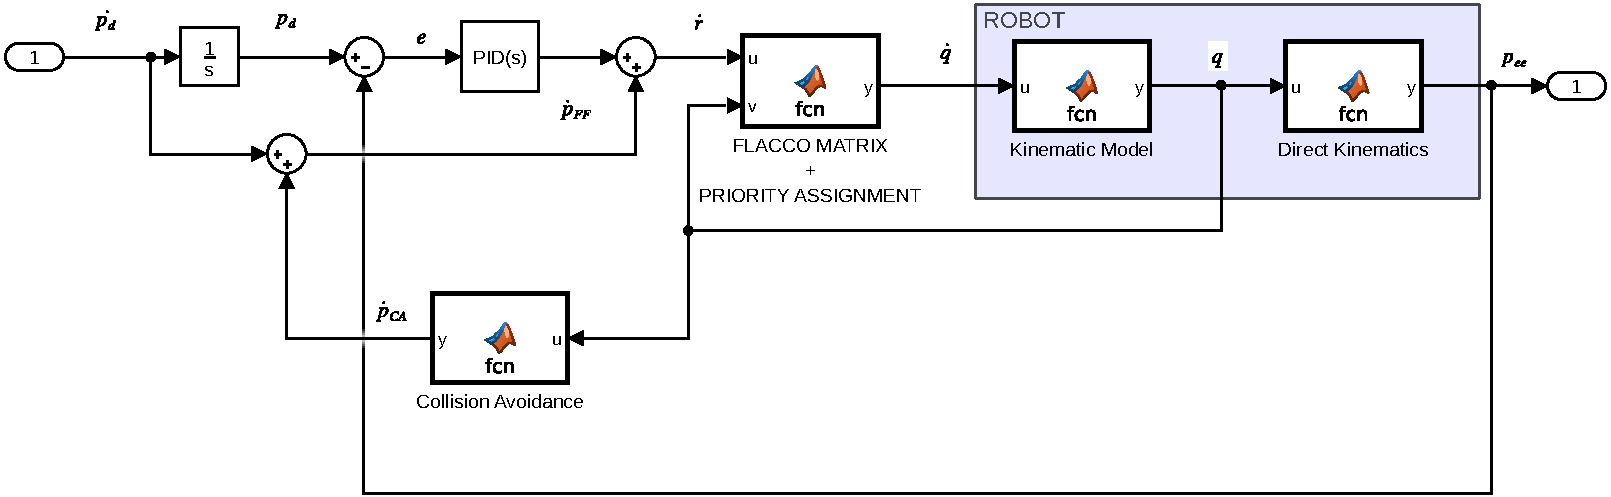
\includegraphics[width = \linewidth]{./plots/ControlSchemeModel.pdf}
\caption{Block scheme of the control architecture.}
\end{figure*}
Which is a feedback plus feed-forward control architecture, where the feed-forward term is designed to achieve collision avoidance for the end-effector.

Note that all the information about the other control points and tasks are included into the \emph{Flacco Matrix} and into the task velocities' vector.
Those quantities have not been included since they are "known" at the control architecture's level and require no external reference.
\section{Code}

\section{Results}

\bibliography{sample}
\bibliographystyle{ieeetr}
\tableofcontents
\end{document}
